Programe en su lenguaje favorito.
Necesitará (al menos) funciones que hagan lo siguiente:
\begin{itemize}
	\item Generar una secuencia aleatoria de 200 bases
		equiprobables e independientes.
		Nos interesa la evolución de una especie alienígena
		en que las bases del DNA son 6, no 4: $A,C,G,T,B,D$.

	\item Una función que aplique una mutación a una secuencia;
		la mutación se escoge entre inserción, borrado y reemplazo
		de manera equiprobable, y su lugar de aplicación se elige
		al azar a lo largo de la secuencia.

		\begin{itemize}
			\item El borrado borra una letra,
			\item la inserción inserta una letra (equiprobable),
			\item el reemplazo reemplaza una letra por cualquiera
				de las otras 5 (de manera equiprobable).
		\end{itemize}

	\item Una función que calcule la distancia de Levenshtein
		entre dos secuencias (implementando Needleman-Wunsch).
\end{itemize}

Con esas funciones, hará lo siguiente:

\red{Importante:} Las funciones y los algoritmos para cada pregunta se encuentran en el Anexo I~\ref{sec:anexo1}.

\begin{enumerate}

	\item Generar una secuencia, y aplicar M mutaciones; para M entre 0 y 300, grafique la relación
		entre M y D, donde D es la distancia de Levenshtein entre la secuencia final y la secuencia
		inicial.

		\blue{Respuesta:}

		\begin{center}
			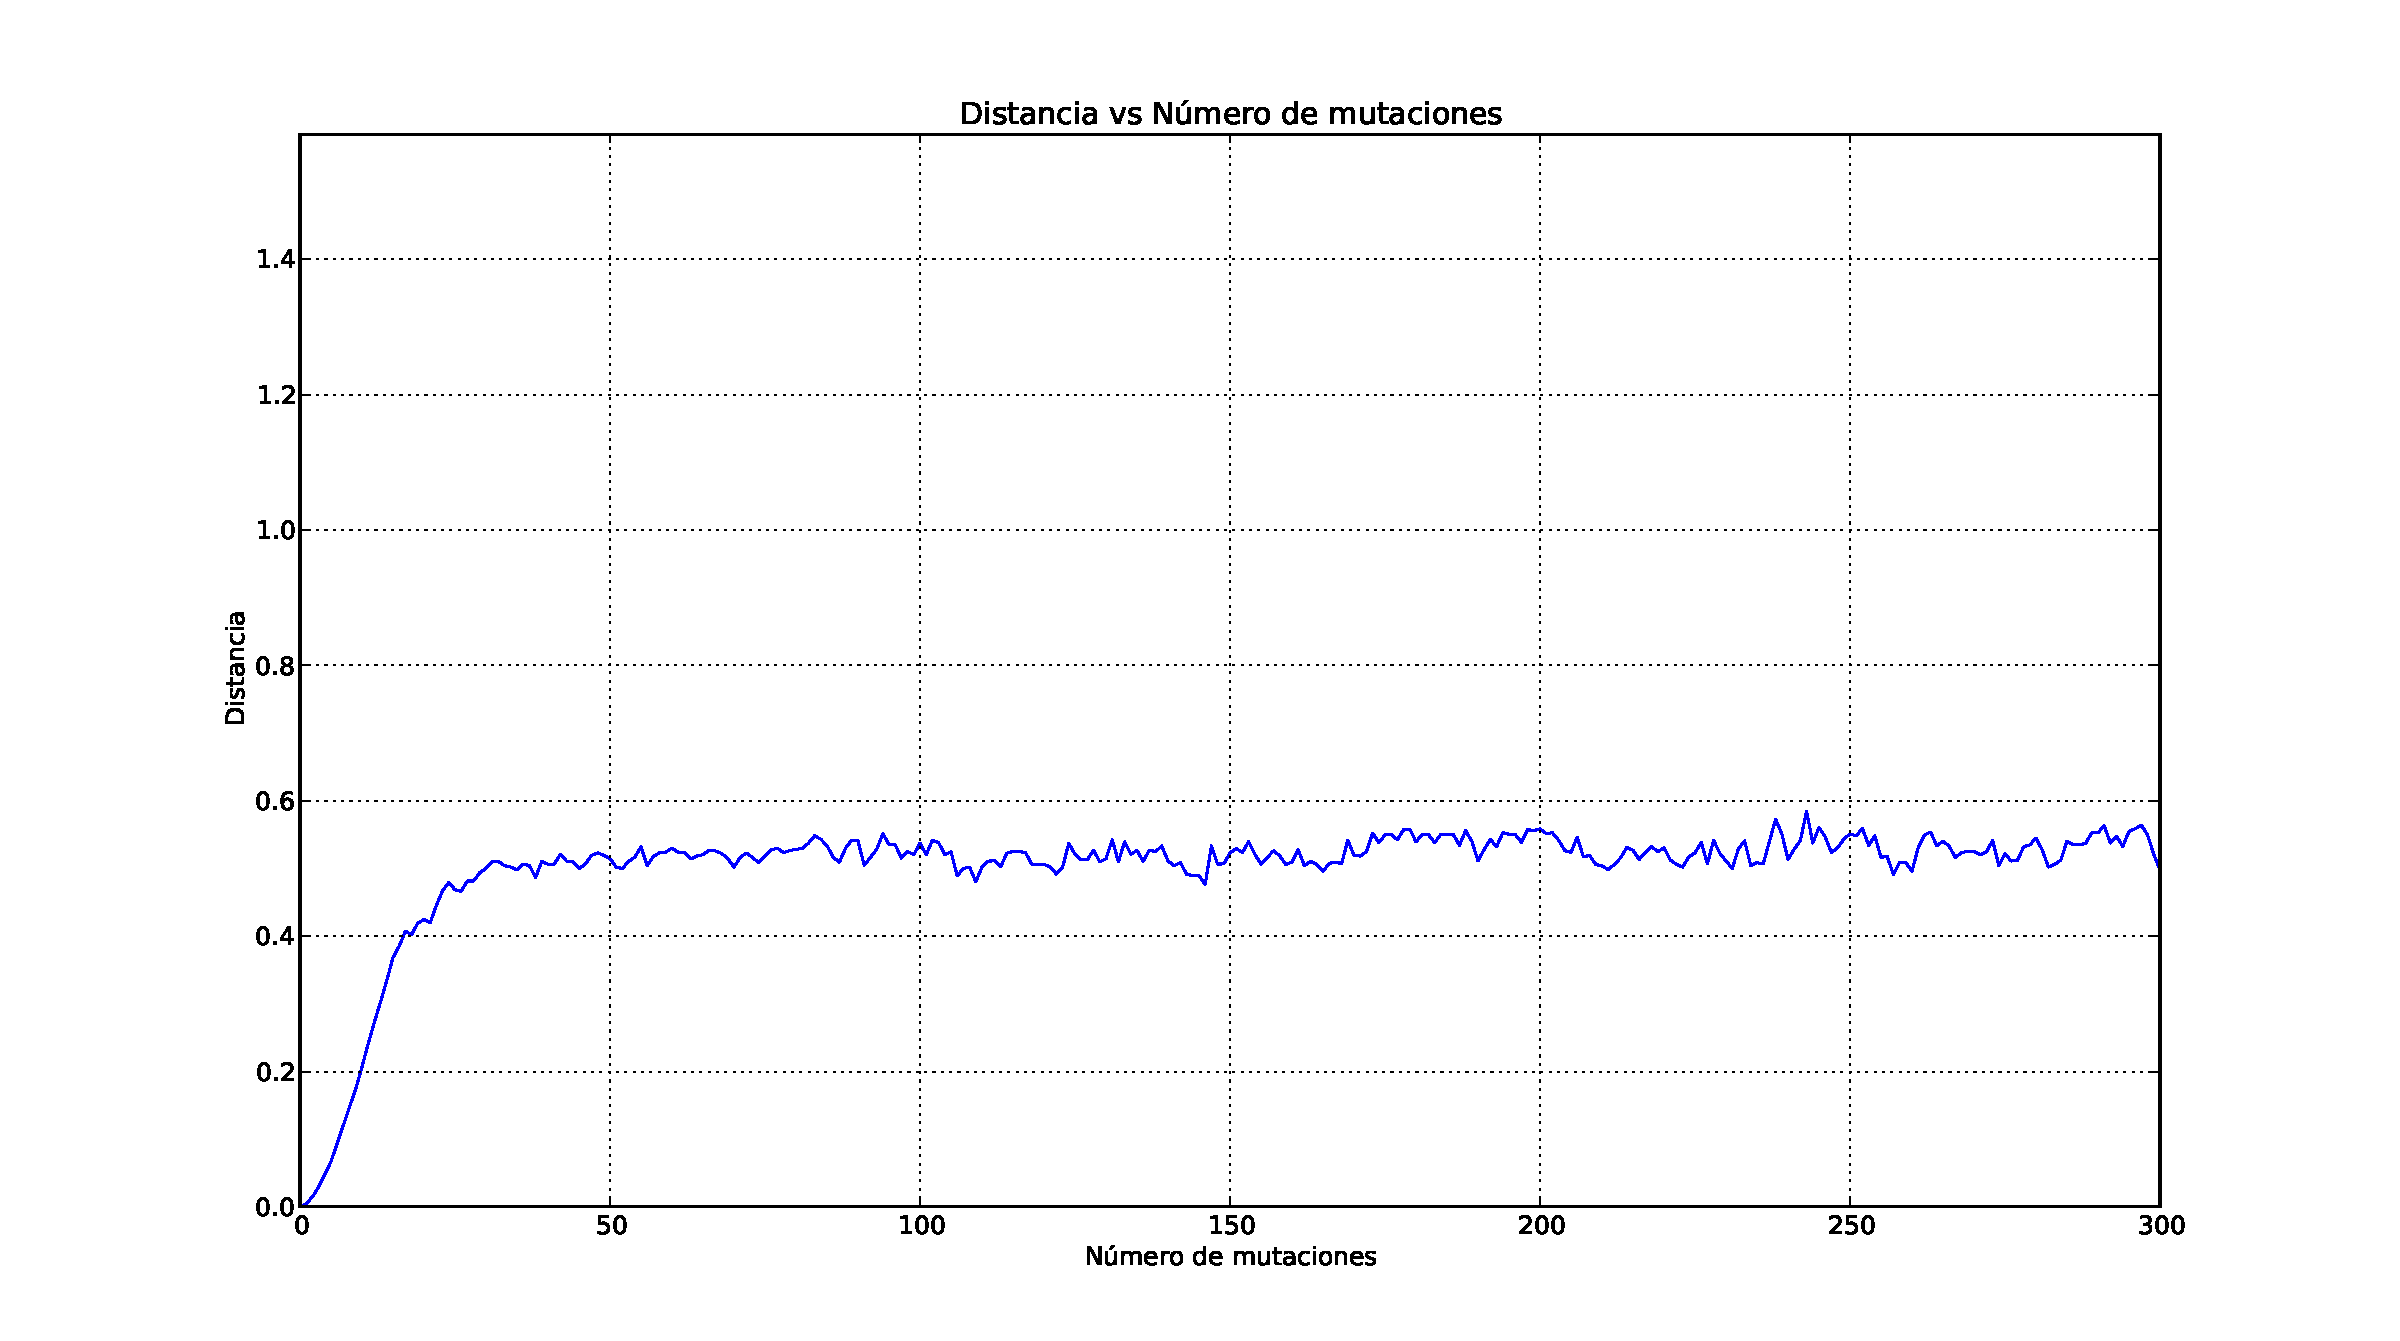
\includegraphics[width=\textwidth]{scripts/pregunta-2-1-new.pdf}
		\end{center}


	\item Genere una secuencia, clónela, y a cada copia aplíquele M mutaciones (de modo que tendrá
		dos secuencias crecientemente distintas). Grafique la relación entre M y D’, donde D’ es la
		distancia entre las dos secuencias que están mutando.

		\blue{Respuesta:}

		\begin{center}
			\includegraphics[width=\textwidth]{scripts/pregunta-2-2-new.pdf}
		\end{center}


	\item Genere 10.000 pares de secuencias (largo 200 c/u) y evalúe su distancia de Levenshtein; haga
		un histograma de la distribución de estos valores, y calcule media y $\sigma$

		\blue{Respuesta:}

		\begin{center}
			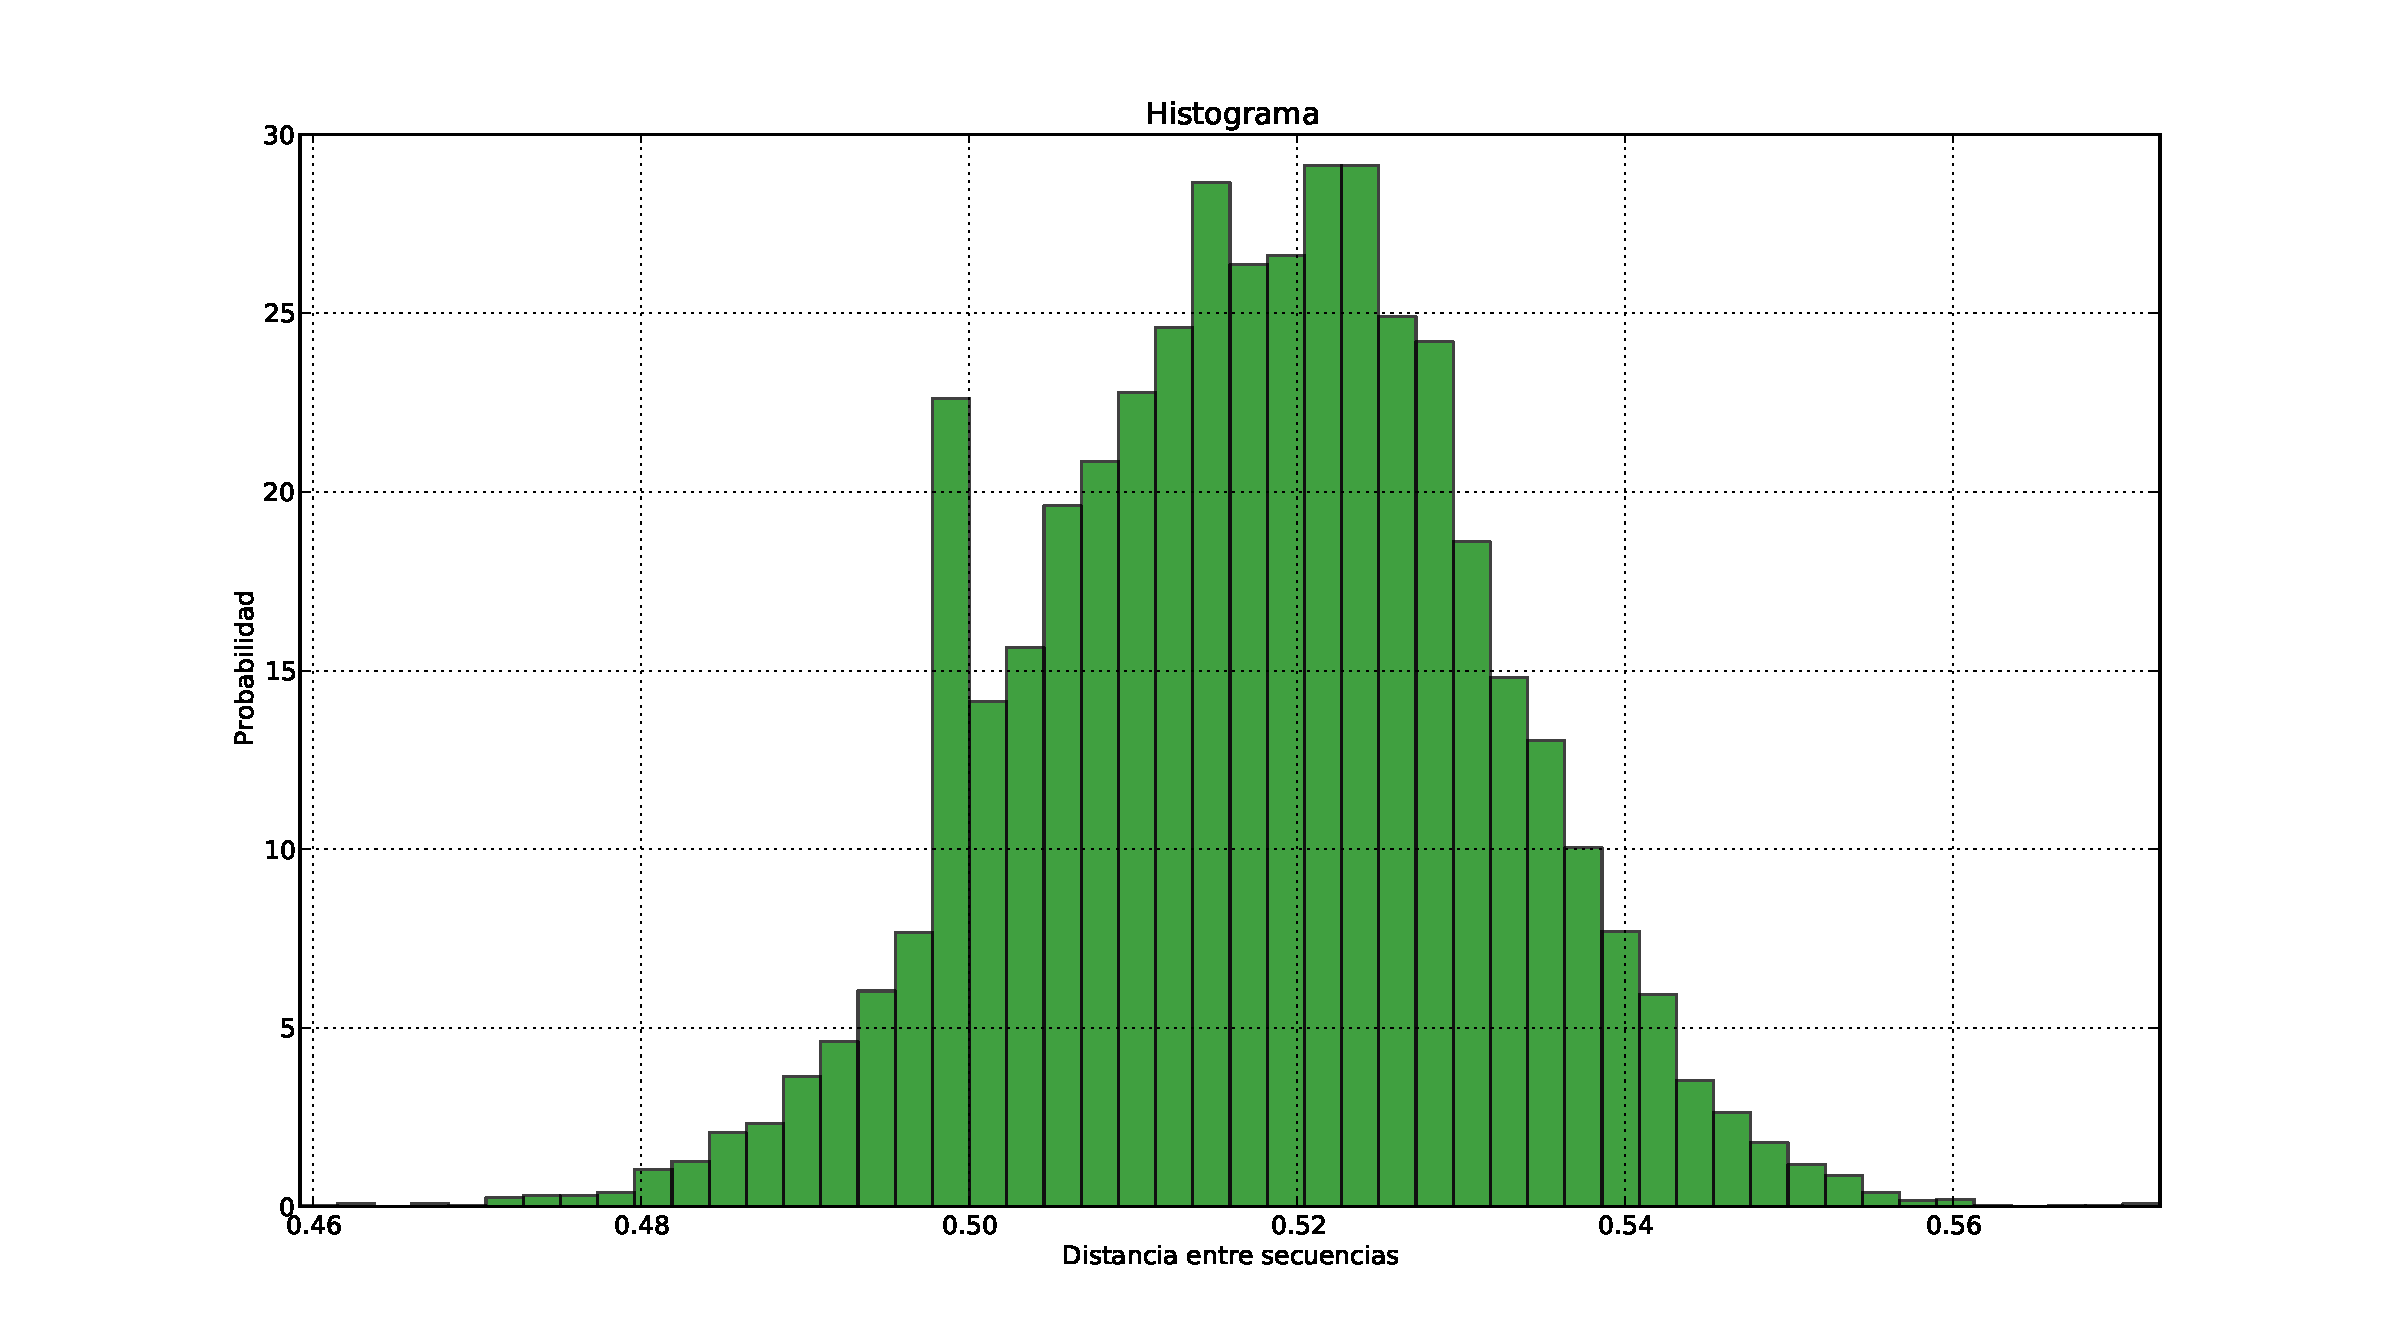
\includegraphics[width=\textwidth]{scripts/pregunta-2-3-new.pdf}
		\end{center}

		La información correspondiente del histograma y la aplicación es la siguiente:

		\begin{center}
		\begin{tabular}{|l|c|}
		\hline
		Largo 			 & 10000   \\\hline
		Media  			 & 0.517 \\\hline
		$\sigma$ 		 & 0.014   \\\hline
		Menor distancia  & 0.459   \\\hline
		Mayor distancia  & 0.573   \\\hline
		Tiempo ejecución & 4140.56 [sec] \\\hline
		\end{tabular}
		\end{center}

	\item Considerando (b) y (c), ¿por sobre qué valor de M diría usted que el parentesco entre las
		secuencias es indetectable?

		\blue{Respuesta:}

		Tomando en cuenta de que cada pregunta tiene sólo la idea central en común,
		es decir calcular la distancia de Levenshtein, pero después de todo,
		los ejercicios son distintos, pues el primero tiene que ver en ir comparando
		dos secuencias que van mutando en conjunto, y el segundo en 10000 pares de
		secuencias independientes que van mutando.

		La información que nos entregará cada ejercicio es la siguiente:
		\begin{itemize}
			\item \emph{(b):} Distancia entre dos secuencias a medida que se van mutando.
			\item \emph{(c):} Distribución de las distancias obtenidas entre 10000 pares de
				secuencias.
		\end{itemize}

		En el caso de la parte \emph{(b)} podemos ver que hasta las \red{30 mutaciones}
		hay una especie de crecimiento lineal, pero luego el comportamiento se torna
		mucho más impreciso, por lo que vamos obteniendo valores en la distancia
		sobre \blue{0.4}, pero a pesar de ser valores distintos, van siguiendo un mismo
		comportamiento, que es muy similar a la función de logaritmo, por lo que podríamos
		decir que la distancia normalizada posee un comportamiento casi logarítmico.

		Por otro lado, en \emph{(c)} nos podemos ver que la mayor cantidad de distancias
		se encuentra entre \blue{0.49} y \blue{0.54}, por lo que podemos deducir, que
		comparando estas distancias obtenidas con el gráfico de la parte \emph{(b)},
		que sobre unas \red{40 mutaciones}, la distancia comienza a ser mayor,
		por lo cual ya no podremos detectar fácilmente el parentesco entre las secuencias,
		a pesar de que todas las distancias obtenidas son similares.

		Finalmente nos damos cuenta de que las distancias en el caso \emph{(c)} siguen
		una \emph{distribución normal}, a pesar de existir un valor extraño cercano al \emph{0.5}.


\end{enumerate}
